%%% LaTeX Template: Article/Thesis/etc. with colored headings and special fonts
%%%
%%% Source: http://www.howtotex.com/
%%% Feel free to distribute this template, but please keep to referal to http://www.howtotex.com/ here.
%%% February 2011
%%%
%%% Modified January 2016 by CDM

%%%  Preamble
\documentclass[11pt,letterpaper]{article}
\usepackage[margin=1.0in]{geometry}
\usepackage[T1]{fontenc}
\usepackage[bitstream-charter]{mathdesign}
\usepackage[latin1]{inputenc}					
\usepackage{amsmath}						
\usepackage{xcolor}
\usepackage{cite}
\usepackage{hyphenat}
\usepackage{graphicx}
\usepackage{float}
\usepackage{subfigure}
\usepackage{sectsty}
\usepackage[compact]{titlesec} 
\usepackage[tablegrid]{vhistory}
\usepackage{pbox}
\allsectionsfont{\color{accentcolor}\scshape\selectfont}

%%% Definitions
\definecolor{accentcolor}{rgb}{0.0,0.0,0.5} 
\newcommahnd{\teamname}{Nepster}
\newcommand{\productname}{Pocket Self}
\newcommand{\coursename}{CSE 4316: Senior Design I}
\newcommand{\semester}{Summer 2019}
\newcommand{\docname}{Architectural Design Specification}
\newcommand{\department}{Department of Computer Science \& Engineering}
\newcommand{\university}{The University of Texas at Arlington}
\newcommand{\authors}{Utsab Acharya \\ Sandesh Naga \\ Sudip Kandel \\ Tara Gurung \\ Bhaskar Acharya}

%%% Headers and footers
\usepackage{fancyhdr}
	\pagestyle{fancy}						% Enabling the custom headers/footers
\usepackage{lastpage}	
	% Header (empty)
	\lhead{}
	\chead{}
	\rhead{}
	% Footer
	\lfoot{\footnotesize \teamname \ - \semester}
	\cfoot{}
	\rfoot{\footnotesize page \thepage\ of \pageref{LastPage}}	% "Page 1 of 2"
	\renewcommand{\headrulewidth}{0.0pt}
	\renewcommand{\footrulewidth}{0.4pt}

%%% Change the abstract environment
\usepackage[runin]{abstract}			% runin option for a run-in title
%\setlength\absleftindent{30pt}			% left margin
%\setlength\absrightindent{30pt}		% right margin
\abslabeldelim{\quad}	
\setlength{\abstitleskip}{-10pt}
\renewcommand{\abstractname}{}
\renewcommand{\abstracttextfont}{\color{accentcolor} \small \slshape}	% slanted text

%%% Start of the document
\begin{document}

%%% Cover sheet
{\centering \huge \color{accentcolor} \sc \textbf{\department \\ \university} \par}
\vspace{1 in}
{\centering \huge \color{accentcolor} \sc \textbf{\docname \\ \coursename \\ \semester} \par}
\vspace{0.5 in}
\begin{figure}[h!]
	\centering
   	
\includegraphics[width=0.60\textwidth]{images/logo}
\end{figure}
\vspace{0.5 in}
{\centering \huge \color{accentcolor} \sc \textbf{\teamname \\ \productname} \par}
\vspace{0.5 in}
{\centering \large \sc \textbf{\authors} \par}
\newpage


%\vspace{1 in}
%\centerline{January 13th, 2012}
%\newpage

%%% Revision History
\begin{versionhistory}
  	\vhEntry{0.1}{08.01.2019}{SK}{document creation}
  	\vhEntry{0.2}{08.02.2019}{SK|UC|SN|BA|TG}{complete draft}
  	\vhEntry{0.3}{08.02.2019}{SK|UC}{release candidate 1}
  	\vhEntry{1.0}{08.02.2019}{SK|SN|BA}{official release}
  	\vhEntry{1.1}{10.31.2015}{TG|UC}{added design review requests}
\end{versionhistory}
\newpage

%%% Table of contents
\setcounter{tocdepth}{2}
\tableofcontents
\newpage

%%% List of figures and tables (optional)
\listoffigures
\listoftables
\newpage

%%% Document sections
\section{Introduction}

 \item Inventory management is an important part of running business and managing items around us. Traditional practice of managing items for business cost a lot of time and work force for companies. Customers become frustrated when the items they’re looking for aren’t available on the shelf. Bad practice of managing items in our home, school, works etc.  cost lots of time because it is hard for us to remember what items are needed and where it is located. Pocket-self is the inventory tracking IOS/Android based mobile application which allow users to keep the items in available space, which is created by the user. We called PocketShelf because the idea behind it, we can carry the inventory application in our pocket and can search items in just a click. The function of the app is user can sign up and login then add items or add shelf or search the items.
 
\item\item App can help to find the place where to keep the items in shelf, keeps record of it and help to find the items when customers search for it. The app can help the customers to find and add the items in the shelf with the help of the item’s pictures too. We used Augmented reality as our key feature of the application. Where user can see the item before they approach to grab it. Which might be helpful in the sense that it will save the user effort and time spent and they know that they are getting the right thing. Time frame to notify user can be pre-defined by the user at the time of its entry. Our app use the online database to save every entry by the user and had to be encrypted before it goes to the database, all the data had to flow through the server. So, user must be online to be able to use the app. We had PIN protection as an extra feature on the app, where if the user wants not to show the item location to another user using the same app on same device. Which we found cool feature if the user wants to secure valuable items somewhere in the shelf.

\item\item The scope of pocketShelf are prioritize inventory, Track all product information, Track sales, sorts inventory according to manufacture and best by date of the items. App helps to prioritize inventory on the basic of the customers demand, shape and sizes of items in the shelf. For example, heavy and big items are preferred in he button of the shelf and small or light items in the top the shelf. App will keep the records of the inventory as well as items in stocks. Another important feature of the app is track sales. Update the numbers of the items when add or remove an item from the shelf. App can sort the inventory according to customer preferences based on attributes of the item. The app not only keep track of the item but able to sort the items based on the expiration dates and can notify the user if the item is expiring soon.






\newpage
\section{System Overview}
PocketShelf is an inventory IOS/Android application. Our application consist of many features among which adding item/shelf, search item for each user with Augmented reality experience is the key feature of our application. Diagram below show the overall high level feature of our application.


\begin{figure}[h!]
	\centering
 	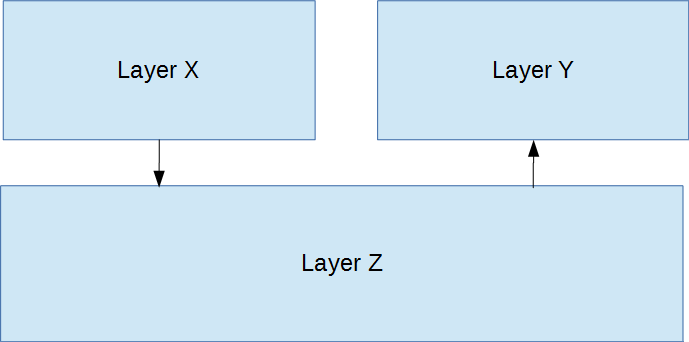
\includegraphics[width=0.60\textwidth]{images/layers}
 \caption{A simple architectural layer diagram}
\end{figure}

\subsection{Layer X Description}
Each layer should be described separately in detail. Descriptions should include the features, functions, critical interfaces and interactions of the layer. The description should clearly define the services that the layer provides. Also include any conventions that your team will use in describing the structure: naming conventions for layers, subsystems, modules, and data flows; interface specifications; how layers and subsystems are defined; etc. 

\subsection{Layer Y Description}
Each layer should be described separately in detail. Descriptions should include the features, functions, critical interfaces and interactions of the layer. The description should clearly define the services that the layer provides. Also include any conventions that your team will use in describing the structure: naming conventions for layers, subsystems, modules, and data flows; interface specifications; how layers and subsystems are defined; etc. 

\subsection{Layer Z Description}
Each layer should be described separately in detail. Descriptions should include the features, functions, critical interfaces and interactions of the layer. The description should clearly define the services that the layer provides. Also include any conventions that your team will use in describing the structure: naming conventions for layers, subsystems, modules, and data flows; interface specifications; how layers and subsystems are defined; etc. 
\newpage
\section{Subsystem Definitions \& Data Flow}


\begin{figure}[h!]
	\centering
 	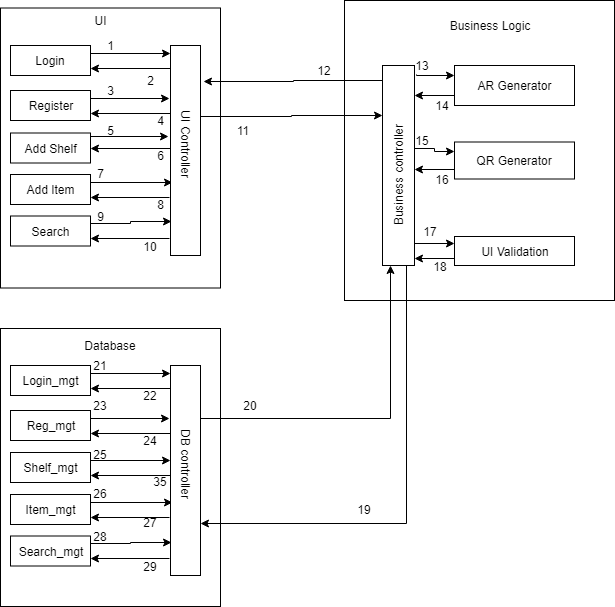
\includegraphics[width=\textwidth]{images/dataflow}
 \caption{A simple data flow diagram}
\end{figure}

\newpage
\section{User Interface (UI)}
This is the first sub section that user interacts with. When the user opens the mobile application for the first time details for SignUp is displayed. Then the user enters all the information required for SignUp including all the valid user name and password to create a account. Then an account for the user is created.

\subsection{UI Controller}


\begin{figure}[h!]
	\centering
 	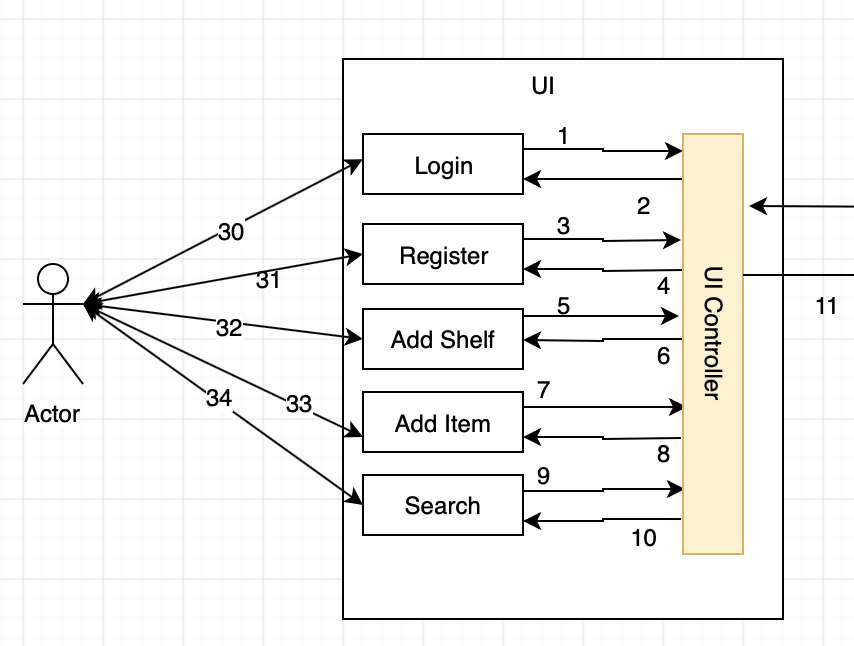
\includegraphics[width=0.60\textwidth]{images/uicontroller}
 \caption{UI Controller description diagram}
\end{figure}

\subsubsection{Assumptions}
Following assumptions are made for this SubSystem:
\begin{itemize}
    \item 
\end{itemize}

\subsubsection{Responsibilities}
Following are the responsibilities of this SubSystem:
\begin{itemize}
    \item 
\end{itemize}

\subsubsection{Subsystem Interfaces}
Each of the inputs and outputs for the subsystem are defined here. Create a table with an entry for each labelled interface that connects to this subsystem. For each entry, describe any incoming and outgoing data elements will pass through this interface.

\begin {table}[H]
\caption {Subsystem interfaces} 
\begin{center}
    \begin{tabular}{ | p{1cm} | p{6cm} | p{3cm} | p{3cm} |}
    \hline
    ID & Description & Inputs & Outputs \\ \hline
    \#xx & Description of the interface/bus & \pbox{3cm}{input 1 \\ input 2} & \pbox{3cm}{output 1}  \\ \hline
    \#xx & Description of the interface/bus & \pbox{3cm}{N/A} & \pbox{3cm}{output 1}  \\ \hline
    \end{tabular}
\end{center}
\end{table}

\subsection{Login}


\begin{figure}[h!]
	\centering
 	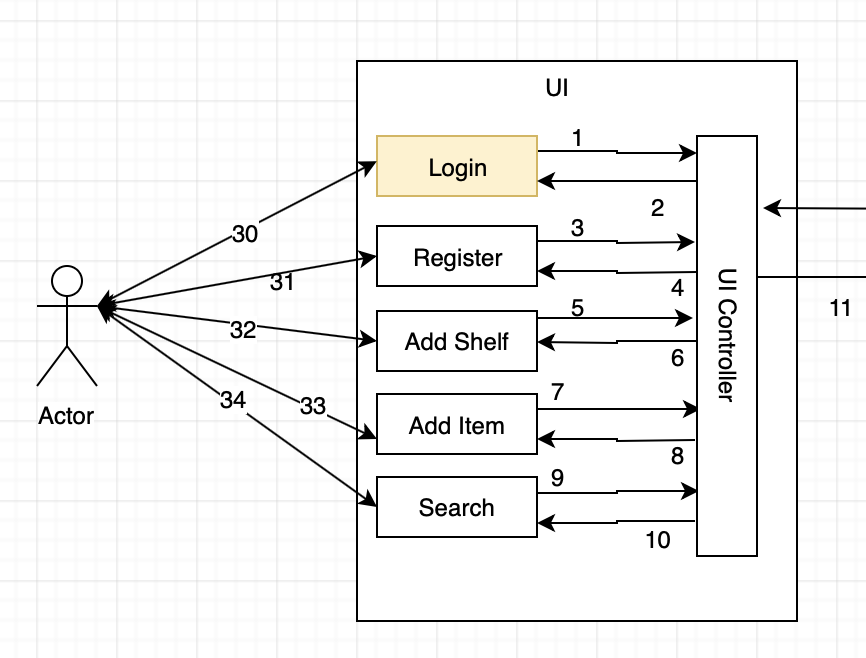
\includegraphics[width=0.60\textwidth]{images/login}
 \caption{Login description diagram}
\end{figure}

\subsubsection{Assumptions}
Following assumptions are made about this SubSystem:
\begin{itemize}
    \item User clicked on the login or signup button in the home screen.
    \item Users cellphone is connected to the internet.
    \item User has a valid Email address.
    \item User provides the password that satisfies the basic password constrain
\end{itemize}

\subsubsection{Responsibilities}
These are the following responsibilities of this subsystem:
\begin{itemize}
    \item Email address must be validated. If Email address doesn’t exist or is not valid, SubSystem must prevent from creating or acessing the account.
    \item If the password doesn’t meet minimum criteria, SubSystem must prevent user form creating account.
\end{itemize}

\subsubsection{Subsystem Interfaces}
Each of the inputs and outputs for the subsystem are defined here. An entry for each labelled interface that connects to this subsystem is shown in the table below:

\begin {table}[H]
\caption {Subsystem interfaces} 
\begin{center}
    \begin{tabular}{ | p{1cm} | p{6cm} | p{3cm} | p{3cm} |}
    \hline
    ID & Description & Inputs & Outputs \\ \hline
    \#1 & User Login Information & \pbox{3cm}{Username Password} & \pbox{3cm}{Login Confirmation msg}  \\ \hline
    \#2 & Login & \pbox{3cm}{N/A} & \pbox{3cm}{msg from UI Controller}  \\ \hline
    \end{tabular}
\end{center}
\end{table}

\subsection{Register}


\begin{figure}[h!]
	\centering
 	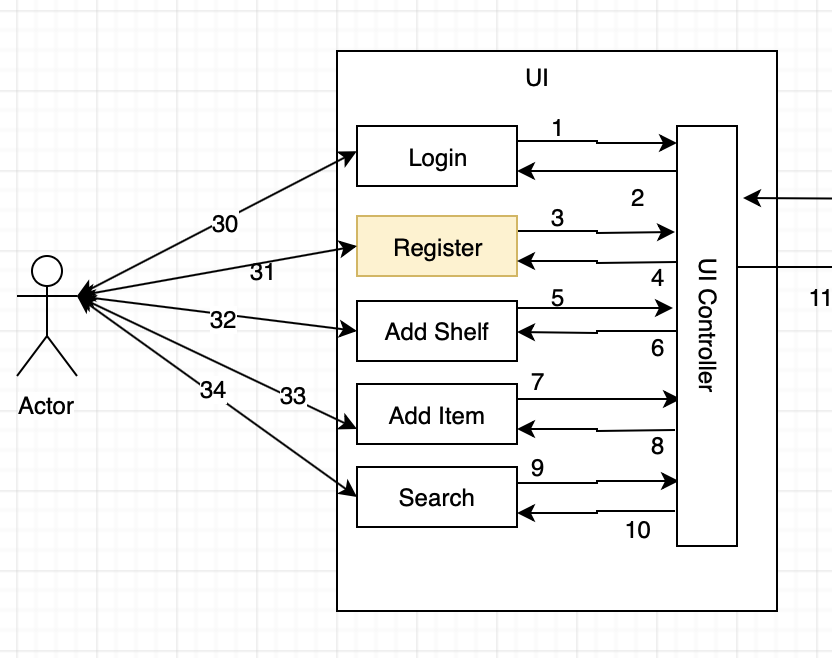
\includegraphics[width=0.60\textwidth]{images/register}
 \caption{Register description diagram}
\end{figure}

\subsubsection{Assumptions}
Following are the assumption of SubSection Email/Password Validation:
\begin{itemize}
    \item User clicked on the register button.
    \item Users cellphone is connected to the internet.
    \item The user inputs all the information in the sign up form.
    \item The User ID and Password input is valid meeting the minimum criteria.
\end{itemize}
\subsubsection{Responsibilities}
Following responsibilities must be carried out by this SubSystem:
\begin{itemize}
    \item Email address, user name and the password is validated. If the provided email address is not valid then user is not allowed to register for the account.
    \item The system must only accept a unique username and a unique email address.
    \item User password must satisfy minimum criteria for the assword constrain.
\end{itemize}

\subsubsection{Subsystem Interfaces}
Each of the inputs and outputs for the subsystem are defined here. Create a table with an entry for each labelled interface that connects to this subsystem. For each entry, describe any incoming and outgoing data elements will pass through this interface.

\begin {table}[H]
\caption {Subsystem interfaces} 
\begin{center}
    \begin{tabular}{ | p{1cm} | p{6cm} | p{3cm} | p{3cm} |}
    \hline
    ID & Description & Inputs & Outputs \\ \hline
    \#3 & Register & \pbox{3cm}{user} & \pbox{3cm}{user information}  \\ \hline
    \#4 & Register & \pbox{3cm}{N/A} & \pbox{3cm}{msg from the controller}  \\ \hline
    \end{tabular}
\end{center}
\end{table}


\subsection{Add Shelf}


\begin{figure}[h!]
	\centering
 	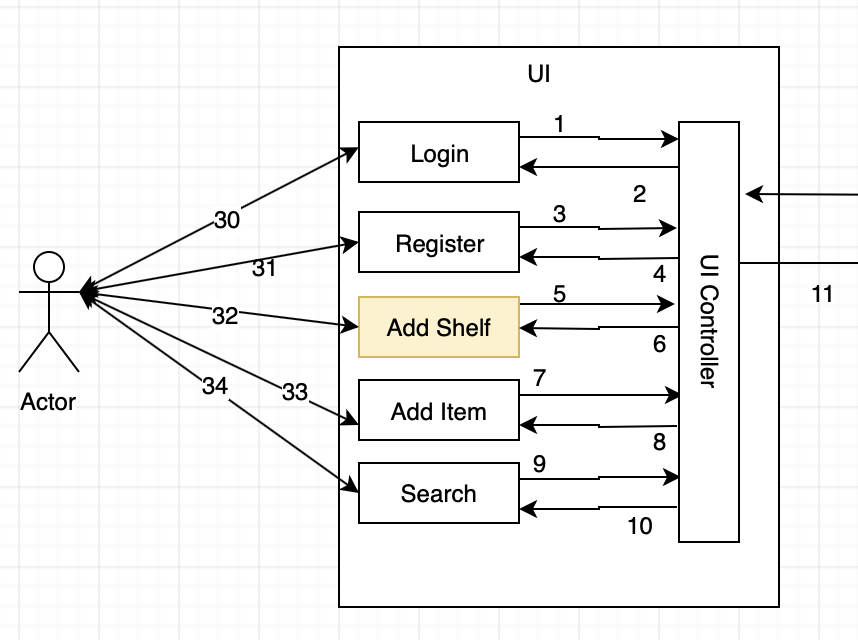
\includegraphics[width=0.60\textwidth]{images/addshelf}

 \caption{Adding Shelf description diagram}

\end{figure}

\subsubsection{Assumptions}
Following assumptions are made about this SubSystem:
\begin{itemize}
    \item User clicked on the add shelf button
    \item Users cellphone is connected to the internet.
    \item User inputs all the information required to create a new shelf
    \item User inputs a valid measurement dimensions.
\end{itemize}

\subsubsection{Responsibilities}
These are the following responsibilities of this subsystem:
\begin{itemize}
    \item The system validate the measurement.
\end{itemize}

\subsubsection{Subsystem Interfaces}
Each of the inputs and outputs for the Add shelf subsystem are defined here.

\begin {table}[H]
\caption {Subsystem interfaces} 
\begin{center}
    \begin{tabular}{ | p{1cm} | p{6cm} | p{3cm} | p{3cm} |}
    \hline
    ID & Description & Inputs & Outputs \\ \hline
    \#5 & Add shelf & \pbox{3cm}{user} & \pbox{3cm}{Shelf information}  \\ \hline
    \#6 & Add shelf & \pbox{3cm}{N/A} & \pbox{3cm}{msg from the UI controller}  \\ \hline
    \end{tabular}
\end{center}
\end{table}

\subsection{Add Item}
Add Item allows the user to add the items with the description of its different attributes. Attributes like name of product, brand name, manufacture date, best by date and size of product.


\begin{figure}[h!]
	\centering
 	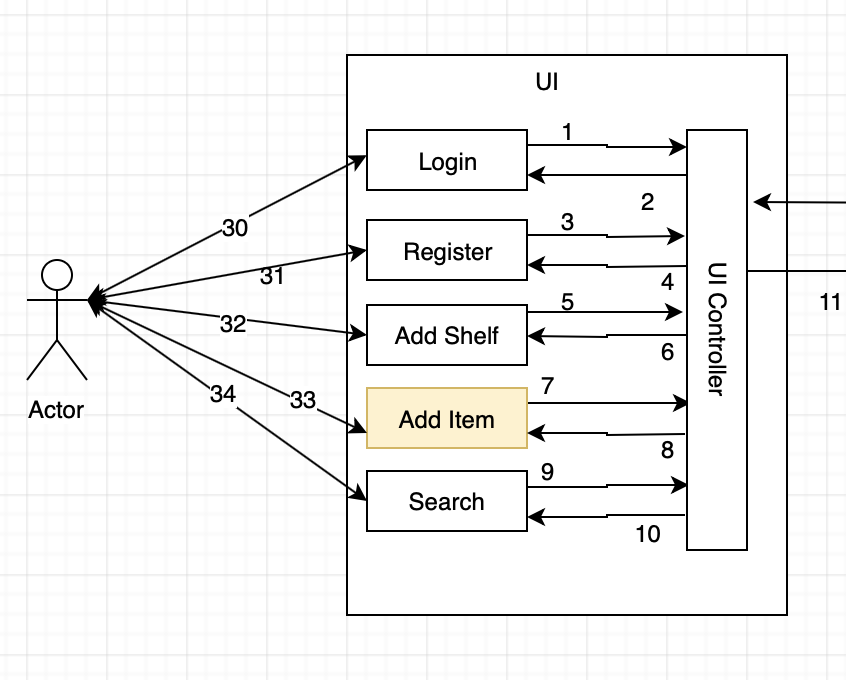
\includegraphics[width=0.60\textwidth]{images/additem}

 \caption{Adding items description diagram}

\end{figure}

\subsubsection{Assumptions}
Following assumptions are made about this SubSystem:
\begin{itemize}
    \item User clicked on add item button
    \item Users cell phone is connected to the internet
    \item User input detailed description about the item.
\end{itemize}

\subsubsection{Responsibilities}
These are the following responsibilities of this subsystem:
\begin{itemize}
    \item The system must get the detailed information from the user and send it to the UI Controller.
\end{itemize}

\subsubsection{Subsystem Interfaces}
Each of the inputs and outputs for the subsystem are defined here. Create a table with an entry for each labelled interface that connects to this subsystem. For each entry, describe any incoming and outgoing data elements will pass through this interface.

\begin {table}[H]
\caption {Subsystem interfaces} 
\begin{center}
    \begin{tabular}{ | p{1cm} | p{6cm} | p{3cm} | p{3cm} |}
    \hline
    ID & Description & Inputs & Outputs \\ \hline
    \#7 & Add Item & \pbox{3cm}{user} & \pbox{3cm}{Item Information}  \\ \hline
    \#8 & Add Item & \pbox{3cm}{N/A} & \pbox{3cm}{msg from the controller}  \\ \hline
    \end{tabular}
\end{center}
\end{table}

\subsection{Search}


\begin{figure}[h!]
	\centering
 	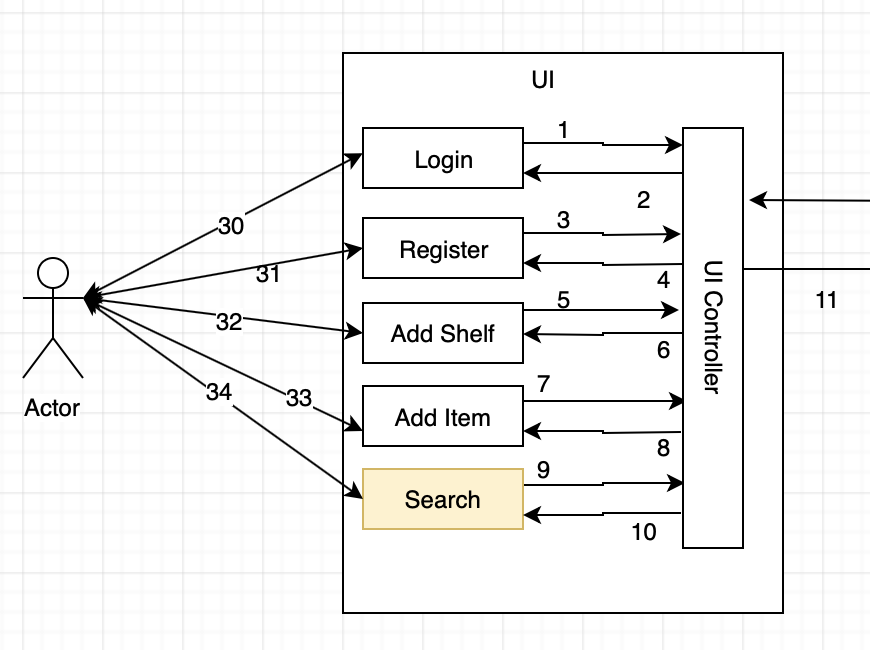
\includegraphics[width=0.60\textwidth]{images/search}
 \caption{searching item description diagram}
\end{figure}

\subsubsection{Assumptions}
Following assumptions are made about this SubSystem:
\begin{itemize}
    \item User clicked on the search button
    \item Users cell phone is connected to the internet
    \item User search for the item with either bar code or manually. If search is with the bar code camera is accessed to scan the bar code and if the search is manual then a text entry field is available.
\end{itemize}

\subsubsection{Responsibilities}
These are the following responsibilities of this subsystem:
\begin{itemize}
    \item The system should be able to get the data from user and send it to the UI Controller.
\end{itemize}

\subsubsection{Subsystem Interfaces}
Each of the inputs and outputs for the subsystem are defined here. Create a table with an entry for each labelled interface that connects to this subsystem. For each entry, describe any incoming and outgoing data elements will pass through this interface.

\begin {table}[H]
\caption {Subsystem interfaces} 
\begin{center}
    \begin{tabular}{ | p{1cm} | p{6cm} | p{3cm} | p{3cm} |}
    \hline
    ID & Description & Inputs & Outputs \\ \hline
    \#9 & Search & \pbox{3cm}{user} & \pbox{3cm}{barcode // text}  \\ \hline
    \#10 & Search & \pbox{3cm}{N/A} & \pbox{3cm}{msg from the UI Controller}  \\ \hline
    \end{tabular}
\end{center}
\end{table}


\newpage
\section{Business Logic}

This is another important layer in our design. This part of the system works as a bridge between the User Interface and the Database of the system. If the data is being received from the UI controller that are coming form different subsections of UI, the Business controller will, depending upon what kind of input it gets, either generate an AR, generate a Qr or does an input validation. The Business Logic will send the data to the data base for more validation and verification or to store the data in database. If Business Logic is getting the instruction to fetch data form Database, then it will contact Database to get particular data, which is then passed on to the UI.

\subsection{Business Controller}
Any kind of data coming and going to Business Logic do so through the Business controller. The data coming to Business Logic will be divided into three different ways, namely AR generation, QR generation or Input Validation related. Depending upon those different input types, Business controller communicates with the Database controller to get particular data or to store that information.

\begin{figure}[h!]
	\centering
 	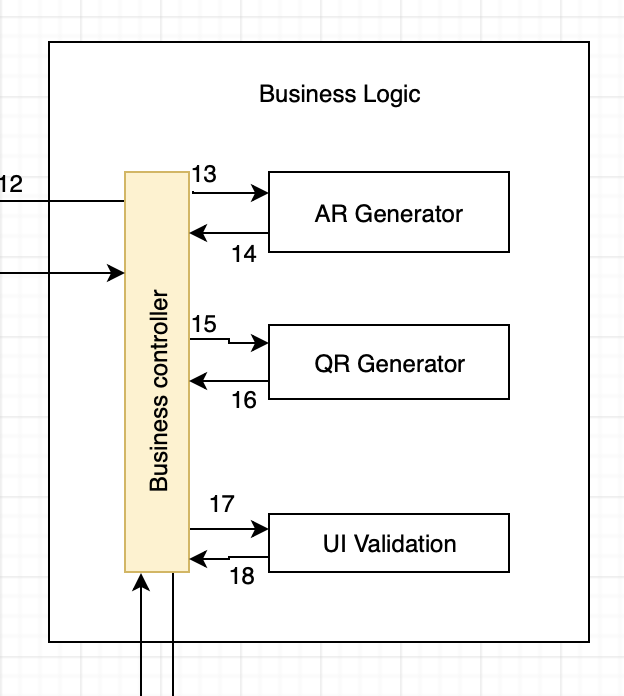
\includegraphics[width=0.60\textwidth]{images/businesscontroller}
 \caption{Example subsystem description diagram}
\end{figure}

\subsubsection{Assumptions}

\begin{itemize}
    
    \item UI is working fine and UI controller has well established connection with the Business Logic.
    \item Database is working fine and DB controller has well established connection with the Business Logic.
\end{itemize}

\subsubsection{Responsibilities}
Following are the responsibilities of the Business Logic:
\begin{itemize}
    \item Creating QR for any new item to be stored in the inventory.
    \item Creating AR for any new item to be stored in the inventory.
    \item Validate the input coming from the UI.
    \item Send QR generated to be stored in Database.
    \item Send AR generated  to be stored in the Database.
    \item Fetch required data from Database that are required by the UI.
\end{itemize}


\subsubsection{Subsystem Interfaces}
Each of the inputs and outputs for the subsystem are defined here. 

\begin {table}[H]
\caption {Subsystem interfaces} 
\begin{center}
    \begin{tabular}{ | p{1cm} | p{6cm} | p{3cm} | p{3cm} |}
    \hline
    ID & Description & Inputs & Outputs \\ \hline
    \#12 & Business Controller/UI Controller & \pbox{3cm}{Login, Registration, Add item, add Shelf, search data} & \pbox{3cm}{N/A}  \\ \hline
    \#11 & UI Controller/Business Controller & \pbox{3cm}{N/A} & \pbox{3cm}{AR, QR, success/failure Message}  \\ \hline
   
    \#13 & Business Controller/AR Generator & \pbox{3cm}{item description} & \pbox{3cm}{}  \\ \hline
    \#14 & AR GeneratorBusiness/Business Controller & \pbox{3cm}{N/A} & \pbox{3cm}{AR image}  \\ \hline
    
    \#15 & Business Controller/QR Generator & \pbox{3cm}{Item description} & \pbox{3cm}{N/A}  \\ \hline
    \#16 & QR Generator /Business Controller& \pbox{3cm}{N/A} & \pbox{3cm}{QR Code}  \\ \hline
    
    \#17 & Business Controller/UI validation & \pbox{3cm}{User Input} & \pbox{3cm}{N/A}  \\ \hline
    \#18 & UI validation / Business Controller& \pbox{3cm}{N/A} & \pbox{3cm}{Success/Failure Message}  \\ \hline
    \#19 & Business Controller/DB controller & \pbox{3cm}{User Input,QR, QR} & \pbox{3cm}{N/A}  \\ \hline
    \#20 & DB controller/Business Controller & \pbox{3cm}{N/A} & \pbox{3cm}{Success/Failure Message}  \\ \hline
    
    \end{tabular}
\end{center}
\end{table}

\subsection{AR Generator}
AR generator is the part of Business logic that generates AR when a customer wants to store an item to the shelf. The generated AR is then used when the customer wants to search the item. When the customer wants to search an item, he will scan bar-code or enter manually. Then the program will display the AR right on the bar-code of the item. 

\begin{figure}[h!]
	\centering
 	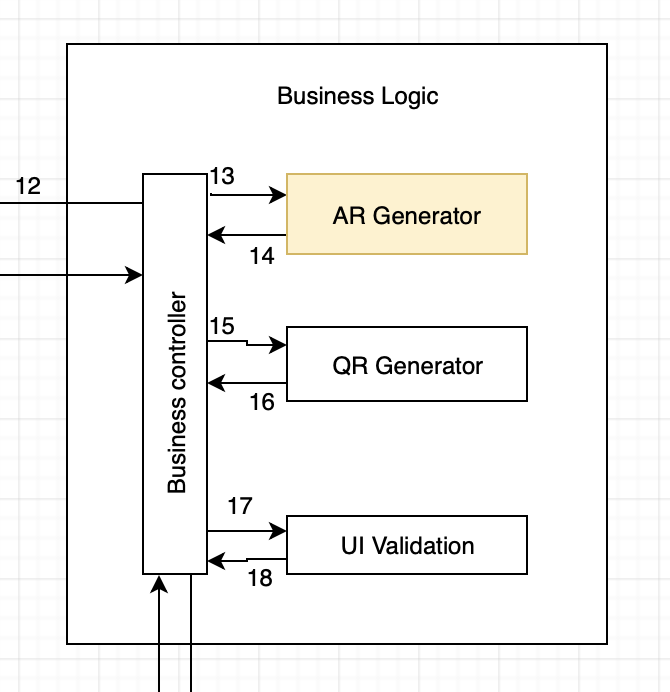
\includegraphics[width=0.60\textwidth]{images/argenerator}
 \caption{AR generator description diagram}
\end{figure}

\subsubsection{Assumptions}
\begin{itemize}
    \item item is in the database
    \item User has a device with working camera.
    \item User has stored valid item image for the item.
\end{itemize}

\subsubsection{Responsibilities}
AR generator produces the AR and when a customer scans a bar-code for the item he is searching, the program will display the AR on the Bar-code.

\subsubsection{Subsystem Interfaces}


\begin {table}[H]
\caption {Subsystem interfaces} 
\begin{center}
    \begin{tabular}{ | p{1cm} | p{6cm} | p{3cm} | p{3cm} |}
    \hline
    ID & Description & Inputs & Outputs \\ \hline
    \#13 & Business Controller/AR Generator & \pbox{3cm}{item description} & \pbox{3cm}{N/A}  \\ \hline
    \#14 & AR GeneratorBusiness/Business Controller & \pbox{3cm}{N/A} & \pbox{3cm}{AR image}  \\ \hline
    \end{tabular}
\end{center}
\end{table}

\subsection{QR Generator}
Based on description of the item customer provides, QR generator generate QR.This QR is then store in the database along with the  description of the item.

\begin{figure}[h!]
	\centering
 	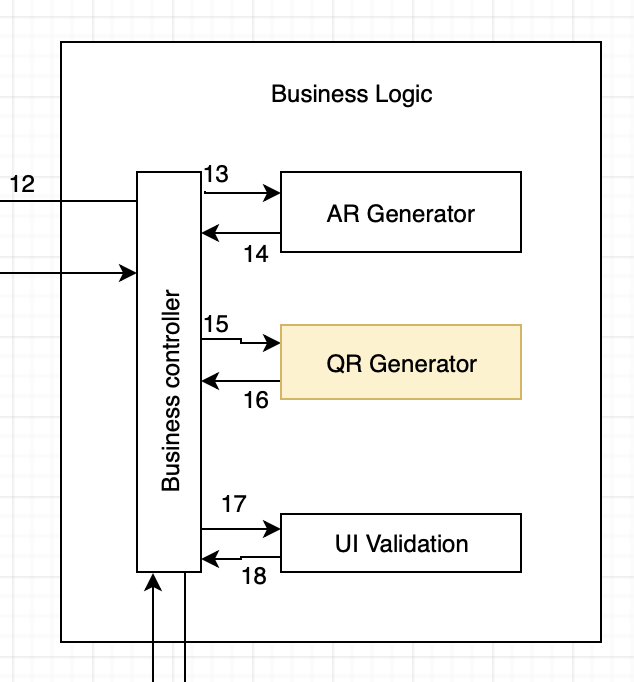
\includegraphics[width=0.60\textwidth]{images/qrgenerator}
 \caption{QR generator description diagram}
\end{figure}

\subsubsection{Assumptions}
\begin{itemize}
    \item Customer inputs the right description of the item to  that is to be stored in inventory.
    \item Item should be new to the inventory.
    
\end{itemize}

\subsubsection{Responsibilities}
QR generator is responsible of generating new QR for each new item that is being added to the inventory. This shall help in giving new identity to the item that is to be stored as well as make it easy to access the item stored in the inventory.

\subsubsection{Subsystem Interfaces}

\begin {table}[H]
\caption {Subsystem interfaces} 
\begin{center}
    \begin{tabular}{ | p{1cm} | p{6cm} | p{3cm} | p{3cm} |}
    \hline
    ID & Description & Inputs & Outputs \\ \hline
    \#15 & Business Controller/QR Generator & \pbox{3cm}{Item description} & \pbox{3cm}{N/A}  \\ \hline
    \#16 & QR Generator /Business Controller& \pbox{3cm}{N/A} & \pbox{3cm}{QR Code}  \\ \hline
    \end{tabular}
\end{center}
\end{table}

\subsection{UI Input Validation}
This section will validate format and types of input from user. It will reject the inputs if user's input is wrong format and suggest the correct format of the input.Provide guidance on how to fix any errors, don't just tell users what they did wrong. It will prevent from unauthorized SQL injection into the data base.
\begin{figure}[h!]
	\centering
 	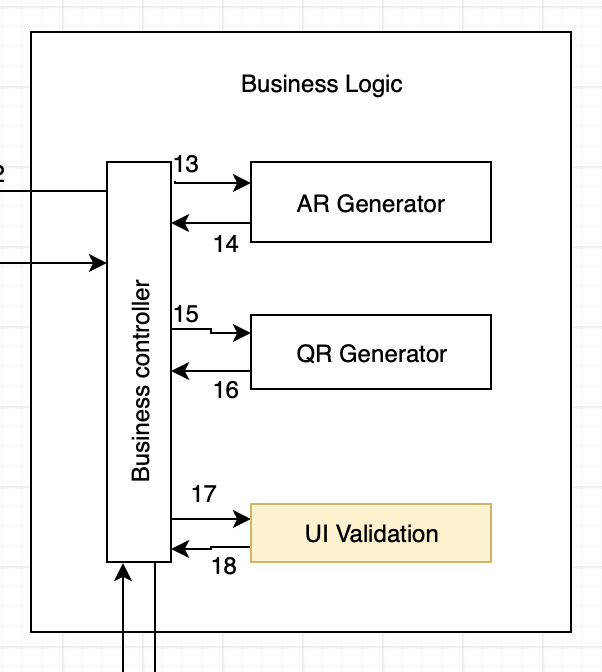
\includegraphics[width=0.60\textwidth]{images/uivalidation}
 \caption{UI Input Validation description diagram}
\end{figure}

\subsubsection{Assumptions}
\begin{itemize}
    \item User input item information.
    \item User has a device with working camera.
    \item User has stored valid item image for the item.
\end{itemize}

\subsubsection{Responsibilities}
Each of the responsibilities/features/functions/services of the subsystem as identified in the architectural summary must be expanded to more detailed responsibilities. These responsibilities form the basis for the identification of the finer-grained responsibilities of the layer's internal subsystems. Clearly describe what each subsystem does.

\subsubsection{Subsystem Interfaces}
Each of the inputs and outputs for the subsystem are defined here. Create a table with an entry for each labelled interface that connects to this subsystem. For each entry, describe any incoming and outgoing data elements will pass through this interface.

\begin {table}[H]
\caption {Subsystem interfaces} 
\begin{center}
    \begin{tabular}{ | p{1cm} | p{6cm} | p{3cm} | p{3cm} |}
    \hline
    ID & Description & Inputs & Outputs \\ \hline
    \#17 & Business Controller/UI validation & \pbox{3cm}{User Input} & \pbox{3cm}{N/A}  \\ \hline
    \#18 & UI validation / Business Controller& \pbox{3cm}{N/A} & \pbox{3cm}{Success/Failure Message}  \\ \hline
    \end{tabular}
\end{center}
\end{table}


\newpage
\section{Database}
This subsection is used when we have to save or retrieve data from the database. When user tries to login, register, add self, add item or search we have to use database. When somebody wants to register for the app, he provides all the information then these information is taken by the DB controller and saved in organized manner. same process occurs for all the other activities like adding self, adding item or login.
\subsection{DB Controller}
This is a type of main controller of the Database system. All the data that needs to be stored in database is first handled by this layer and later stored in the database. When any of the other layer send data to the database layer, first database layer takes the information and figures out what type of data is provided and what to do with the given data.

\begin{figure}[h!]
	\centering
 	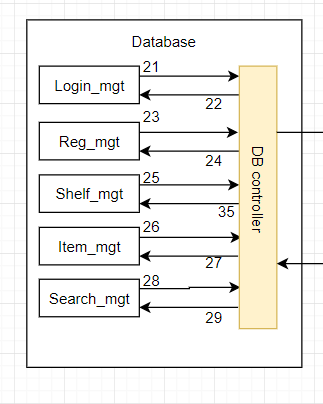
\includegraphics[width=0.60\textwidth]{images/dbcontroller}
 \caption{DB Controller description diagram}
\end{figure}

\subsubsection{Assumptions}
These are the following assumptions made about this subsection:
\begin{itemize}
    \item All the input provided to be saved in the database is a valid input.
    \item Device is connected to the internet when saving or retrieving the data.
\end{itemize}

\subsubsection{Responsibilities}
These are the following responsibilities of the Database Controller.
\begin{itemize}
    \item It must be able to take input sent from all the other layers.  
    \item When input is captured it must be able to classify if the data is login data or sign up data. Must be able to classify if the incoming data is trying to search the item or save the item in the database.
\end{itemize}

\subsubsection{DB Controller Subsystem Interfaces}


\begin {table}[H]
 
\begin{center}
    \begin{tabular}{ | p{1cm} | p{6cm} | p{3cm} | p{3cm} |}
    \hline
    ID & Description & Inputs & Outputs \\ \hline
    \#22 & DB controller/Login\_mgt & \pbox{3cm}{input 1 \\ input 2} & \pbox{3cm}{N/A}  \\ \hline
    \#21 & Login\_mgt/DB Controller & \pbox{3cm}{N/A} & \pbox{3cm}{output 1}  \\ \hline
    
    \#24 & DB Controllere/Reg\_mgt & \pbox{3cm}{input 1 \\ input 2} & \pbox{3cm}{N/A}  \\ \hline
    \#23 & Reg\_mgt/DB Controller & \pbox{3cm}{N/A} & \pbox{3cm}{output 1}  \\ \hline
    
    \#35 & DB Controller/Shelf\_mgt & \pbox{3cm}{input 1 \\ input 2} & \pbox{3cm}{N/A}  \\ \hline
    \#25 & Shel\_mgt/DB Controller & \pbox{3cm}{N/A} & \pbox{3cm}{output 1}  \\ \hline
    
     \#26 & DB Controller/Item\_mgt & \pbox{3cm}{input 1 \\ input 2} & \pbox{3cm}{N/A}  \\ \hline
    \#27 & Item\_mgt/DB Controller & \pbox{3cm}{N/A} & \pbox{3cm}{output 1}  \\ \hline
    
     \#28 & DB Controller/Search\_mgt & \pbox{3cm}{input 1 \\ input 2} & \pbox{3cm}{N/A}  \\ \hline
    \#29 & Search\_mgt/DB Controller & \pbox{3cm}{N/A} & \pbox{3cm}{output 1}  \\ \hline
    \end{tabular}
    \caption {DB Controller Subsystem Interfaces}
\end{center}
\end{table}

\subsection{Login Mgt}
This subsection of database just deals with the login information. User first registers for the account in the mobile application. Then when he wants to use the app he will provide the user name and password for the app. Then the login management layer handles all the data. It checks if the user name and password provided by the user exists in database or not. It should allow user to login if the combination of user name and password exists else it should deny user from using the application itself.

\begin{figure}[h!]
	\centering
 	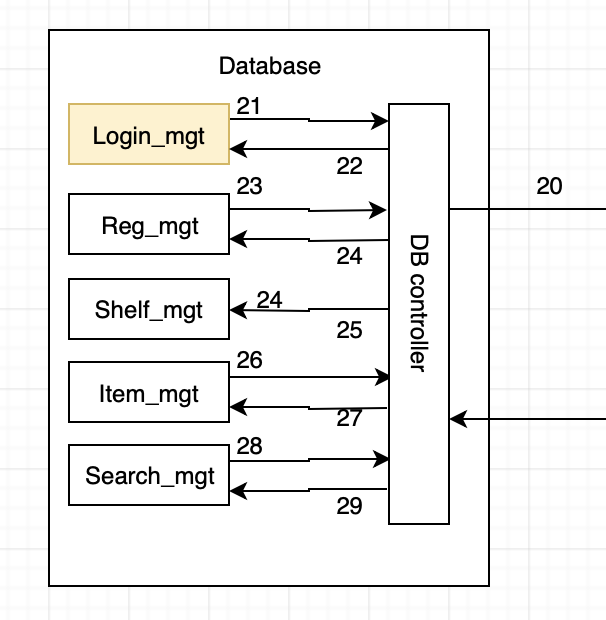
\includegraphics[width=0.60\textwidth]{images/loginmgt}
 \caption{Login mgt description diagram}
\end{figure}

\subsubsection{Assumptions}
These are the following assumptions made about this subsection:
\begin{itemize}
    \item Input provided by the user is valid input. Inputs are not malicious code or SQL query.
\end{itemize}

\subsubsection{Responsibilities}
These are the following responsibilities of this layer;
\begin{itemize}
    \item Check the provided login against the database login information.
    \item If provided login data exists in database let user log in to the app else reject from logging in.
\end{itemize}

\subsubsection{Login Mgt Subsystem Interfaces}
Each of the inputs and outputs for the subsystem are defined here. Create a table with an entry for each labelled interface that connects to this subsystem. For each entry, describe any incoming and outgoing data elements will pass through this interface.

\begin {table}[H]

\begin{center}
    \begin{tabular}{ | p{1cm} | p{6cm} | p{3cm} | p{3cm} |}
    \hline
    ID & Description & Inputs & Outputs \\ \hline
    \#xx & Description of the interface/bus & \pbox{3cm}{input 1 \\ input 2} & \pbox{3cm}{output 1}  \\ \hline
    \#xx & Description of the interface/bus & \pbox{3cm}{N/A} & \pbox{3cm}{output 1}  \\ \hline
    \end{tabular}
    \caption {Login Mgt Subsystem Interfaces} 
\end{center}
\end{table}

\subsection{Register Mgt}
This subsection of the database deals with registration data like first name, last name, DOB,etc. When user provides the information it is validated for SQL injection and passed into the register management. Then the data is stored in database in organized manner by the register management subsystem.

\begin{figure}[h!]
	\centering
 	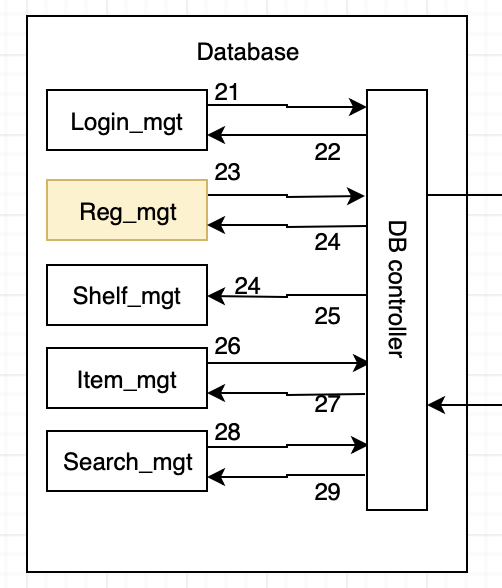
\includegraphics[width=0.60\textwidth]{images/regmgt}
 \caption{Register mgt description diagram}
\end{figure}

\subsubsection{Assumptions}
These are the following assumptions made about this subsection:
\begin{itemize}
    \item User provides all the information needed to register the application. 
    \item Input provided by user is already verified to be the valid input. Eg, malicious code or SQL query is already discarded.
\end{itemize}

\subsubsection{Responsibilities}
These are the following responsibilities of this subsection.
\begin{itemize}
    \item Must be able to return error if all of input field is not provided.
    \item Must be able to store all the information in the database in easy retrieval fashion.
\end{itemize}

\subsubsection{Register Mgt Subsystem Interfaces}
Each of the inputs and outputs for the subsystem are defined here. Create a table with an entry for each labelled interface that connects to this subsystem. For each entry, describe any incoming and outgoing data elements will pass through this interface.

\begin {table}[H]

\begin{center}
    \begin{tabular}{ | p{1cm} | p{6cm} | p{3cm} | p{3cm} |}
    \hline
    ID & Description & Inputs & Outputs \\ \hline
    \#xx & Description of the interface/bus & \pbox{3cm}{input 1 \\ input 2} & \pbox{3cm}{output 1}  \\ \hline
    \#xx & Description of the interface/bus & \pbox{3cm}{N/A} & \pbox{3cm}{output 1}  \\ \hline
    \end{tabular}
    \caption {Register Mgt Subsystem Interfaces} 
\end{center}
\end{table}

\subsection{Shelf mgt}
This subsystem of database is used whenever user wants to add or remove self. When user provides the specification for the self then the database controller takes the data and passes it to the self management layer. Then the layer takes the information and makes the necessary adjustment in the database.
\begin{figure}[h!]
	\centering
 	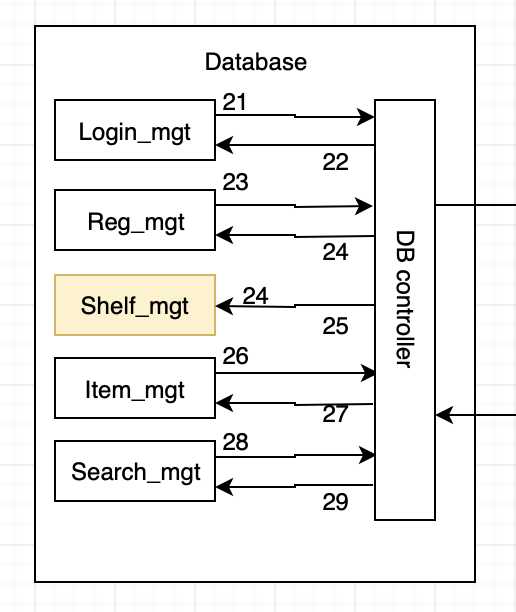
\includegraphics[width=0.60\textwidth]{images/shelfmgt}
 \caption{Shelf mgt description diagram}
\end{figure}

\subsubsection{Assumptions}
These are the following assumptions made about this subsection:
\begin{itemize}
    \item Input provided by user is already verified to be the valid input. Eg, malicious code or SQL query's already discarded.
    \item All the necessary input for adding or deleting the self is provided.
\end{itemize}

\subsubsection{Responsibilities}
These are the following responsibility's that must be performed by this sub system:
\begin{itemize}
    \item Must be able to take all the input values and allocate or de-allocate the self space according to the input values.
\end{itemize}

\subsubsection{Shelf mgt Subsystem Interfaces}
Each of the inputs and outputs for the subsystem are defined here. Create a table with an entry for each labelled interface that connects to this subsystem. For each entry, describe any incoming and outgoing data elements will pass through this interface.

\begin {table}[H]

\begin{center}
    \begin{tabular}{ | p{1cm} | p{6cm} | p{3cm} | p{3cm} |}
    \hline
    ID & Description & Inputs & Outputs \\ \hline
    \#xx & Description of the interface/bus & \pbox{3cm}{input 1 \\ input 2} & \pbox{3cm}{output 1}  \\ \hline
    \#xx & Description of the interface/bus & \pbox{3cm}{N/A} & \pbox{3cm}{output 1}  \\ \hline
    \end{tabular}
    \caption {Shelf mgt Subsystem Interfaces} 
\end{center}
\end{table}

\subsection{Item mgt}
This subsystem of the database is used whenever user wants to add or remove item from the database. When user provides the data for adding or removing the item, then the DB controller takes the input at first and then passes it to the item Mgmt. Then the layer takes the input value and make necessary change ie. add or remove the item accordingly.

\begin{figure}[h!]
	\centering
 	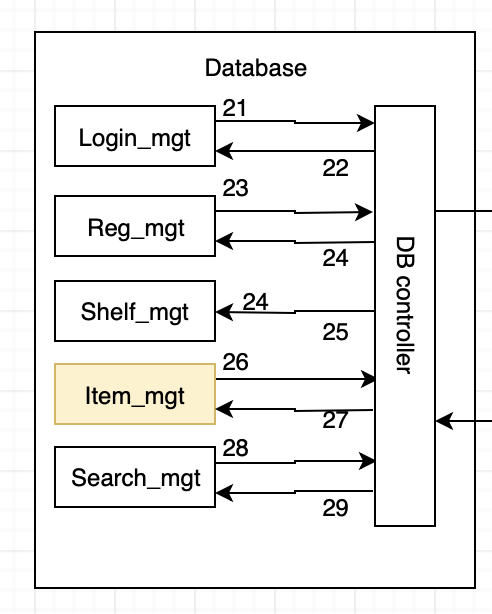
\includegraphics[width=0.60\textwidth]{images/itemmgt}
 \caption{Item mgt description diagram}
\end{figure}

\subsubsection{Assumptions}
These are the following assumptions made about this subsection:
\begin{itemize}
    \item Input provided by user is already verified to be the valid input. Eg, malicious code or SQL query is already discarded.
    \item All the input value is provided by the user.
\end{itemize}

\subsubsection{Responsibilities}
These are the following responsibilities of this subsystem.
\begin{itemize}
    \item Must be able to take all the input values and add or remove item according to the input provided by the user.
\end{itemize}

\subsubsection{Item mgt Subsystem Interfaces}
Each of the inputs and outputs for the subsystem are defined here. Create a table with an entry for each labelled interface that connects to this subsystem. For each entry, describe any incoming and outgoing data elements will pass through this interface.

\begin {table}[H]

\begin{center}
    \begin{tabular}{ | p{1cm} | p{6cm} | p{3cm} | p{3cm} |}
    \hline
    ID & Description & Inputs & Outputs \\ \hline
    \#xx & Description of the interface/bus & \pbox{3cm}{input 1 \\ input 2} & \pbox{3cm}{output 1}  \\ \hline
    \#xx & Description of the interface/bus & \pbox{3cm}{N/A} & \pbox{3cm}{output 1}  \\ \hline
    \end{tabular}
    \caption {Item mgt Subsystem Interfaces} 
\end{center}
\end{table}

\subsection{Search mgt}
This Sub System deals with taking the item description from user and it searches for the item. Variety of options are provided for searching the item. User can use the camera in the cellphone to scan the QR generated for the specific item or users will also be able to search the item by their names.

\begin{figure}[h!]
	\centering
 	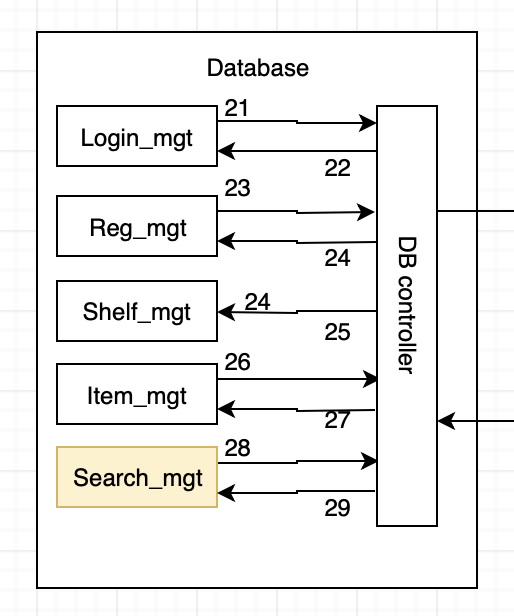
\includegraphics[width=0.60\textwidth]{images/searchmgt}
 \caption{Search mgt description diagram}
\end{figure}

\subsubsection{Assumptions}
These are the following assumptions made about this subsection:
\begin{itemize}
    \item Input provided by user is already verified to be the valid input. Eg, malicious code or SQL query is already discarded.
    \item All the necessary information is provided for the search. 
    \item Device has working camera to scan and search. 
\end{itemize}

\subsubsection{Responsibilities}
These are the following responsibilities of this sub system:
\begin{itemize}
    \item Must be able to take the input and return the result if it exists in database and return "No Items Found" if nothing is found in the database.
\end{itemize}

\subsubsection{Search mgt Subsystem Interfaces}
Each of the inputs and outputs for the subsystem are defined here. Create a table with an entry for each labelled interface that connects to this subsystem. For each entry, describe any incoming and outgoing data elements will pass through this interface.

\begin {table}[H]

\begin{center}
    \begin{tabular}{ | p{1cm} | p{6cm} | p{3cm} | p{3cm} |}
    \hline
    ID & Description & Inputs & Outputs \\ \hline
    \#xx & Description of the interface/bus & \pbox{3cm}{input 1 \\ input 2} & \pbox{3cm}{output 1}  \\ \hline
    \#xx & Description of the interface/bus & \pbox{3cm}{N/A} & \pbox{3cm}{output 1}  \\ \hline
    \end{tabular}
    \caption {Search mgt Subsystem Interfaces} 
\end{center}
\end{table}

\newpage


%%% References
\bibliographystyle{plain}
\bibliographystyle{reference/IEEEtran_custom}
\bibliography{reference/refs}{}

\end{document}